% ch3.tex
% This work is licensed under the Creative Commons Attribution-Noncommercial-Share Alike 3.0 New Zealand License.
% To view a copy of this license, visit http://creativecommons.org/licenses/by-nc-sa/3.0/nz
% or send a letter to Creative Commons, 171 Second Street, Suite 300, San Francisco, California, 94105, USA.


\chapter{Tartarugas e outras criaturas lentas}\index{turtle}\label{ch:turtles}

Existem algumas similaridades entre as tartarugas do mundo real e a do Python. No mundo real, uma tartaruga é um réptil verde, que se move lentamente e carrega sua casa nas suas costas. No mundo do Python, uma tartaruga é uma pequena seta preta que se move lentamente pela tela. Sem se referir à uma casa nas costas.

De fato, considerando que a tartaruga do Python deixa uma trilha e se move pela tela, isso a torna menos parecida com uma tartaruga do mundo real e mais parecida com uma cobra, ou uma lesma. Porém, eu suponho que um módulo chamado `slug' (lesma) não seria muito atraente, então faz sentido continuar com as tartarugas. Imagine uma tartaruga carregando um par de pincéis e desenhando na tela conforme ela anda.

Em um passado profundo, escuro e distante, havia uma simples linguagem de programação chamada Logo. Logo foi usada para controlar uma tartaruga-robô (chamada Irving). Ao longo do tempo, a tartaruga evoluiu de um robô que se movia pelo chão, para uma pequena seta movendo pela tela.

\emph{O que só serve para mostrar que nem sempre as coisas melhoram conforme a tecnologia avança --- uma pequena tartaruga-robô seria muito mais divertido.}

O módulo `turtle' do Python (nós vamos chegar em módulos depois, mas por agora apenas imagine o módulo como algo que nós opdemos usar dentro de um programa) é um pouco como a linguagem de programação Logo, mas enquanto a Logo era (é) bem limitada, o Python possui muito mais recursos. O módulo `turtle' por si só, é um método muito útil para aprender como os computadores desenham figuras no seu monitor.

Vamos começar e ver como isso funciona. O primeiro passo, é dizer ao Python que nós queremos usar o módulo `turtle', importando-o:

\begin{listing}
\begin{verbatim}
>>> import turtle
\end{verbatim}
\end{listing}

Então nós precisamos exibir uma tela para desenhar. Uma tela parecida com a que os artistas usam para pintar; neste caso é um espaço branco para desenhar:

\begin{listing}
\begin{verbatim}
>>> tartaruga = turtle.Pen()
\end{verbatim}
\end{listing}

Nesse código, nós chamamos uma função (Pen\index{Pen}) do módulo `turtle', que automaticamente cria uma tela para nós desenharmos. Uma função é um pedaço de código reutilizável (nós veremos funções mais tarde) que faz algo útil --- neste caso, um objeto que representa uma tartaruga é retornado pela função `Pen' --- nós armazenamos esse objeto na variável `tartaruga'. Quando você digitar o código no terminal do Python, você verá uma tela em branco, assim como na figura~\ref{fig10}.

\begin{figure}
\begin{center}
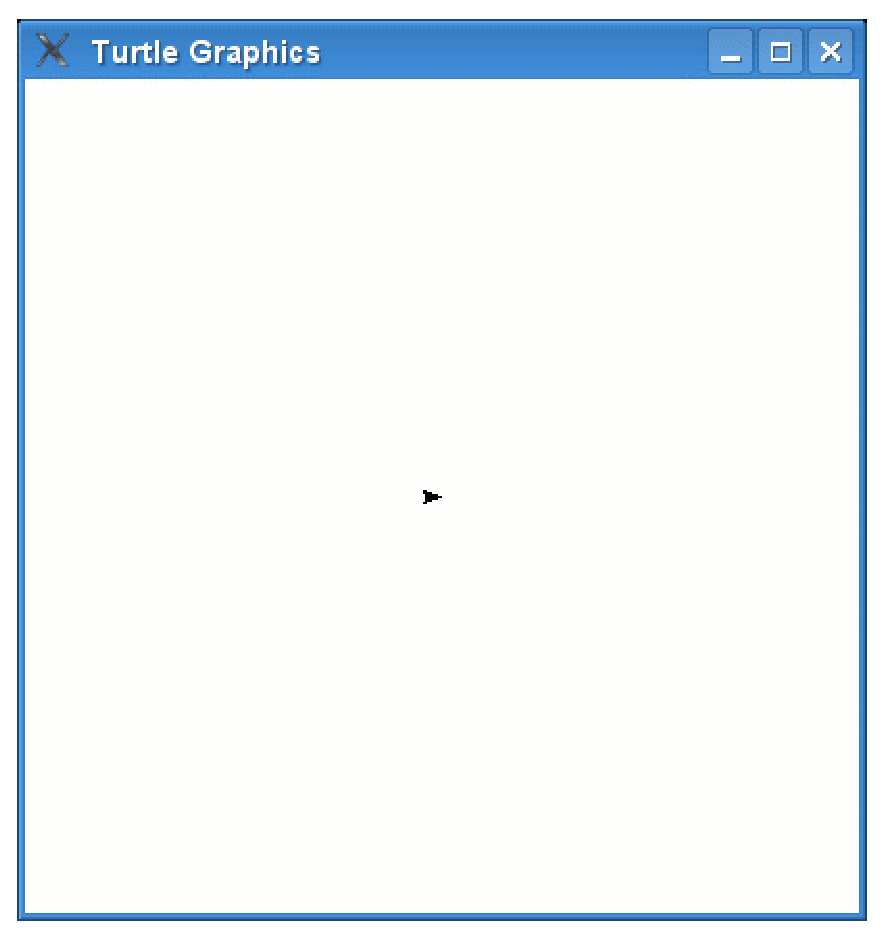
\includegraphics[width=72mm]{eps/figure10.eps}
\end{center}
\caption{Uma seta representando a tartaruga.}\label{fig10}
\end{figure}

\emph{Sim, aquela pequena seta no meio da tela é a nossa tartaruga. E, não, ela não se parece nenhum pouco com uma tartaruga.}

Você pode enviar instruções à tartaruga, usando algumas funções do objeto que nós criamos (chamando \code{turtle.Pen}) --- uma vez que nós atribuimos o objeto à variável \code{tartaruga}, nós usamos \code{tartaruga} para enviar instruções.

Uma das instruções é a \code{forward}. Forward (ir para frente, em português) diz à tartaruga para se mover para frente, seja qual for a direção que ela esteja. Vamos dizer à tartaruga para se mover 40 pixels para frente (nós falaremos sobre pixels em um minuto).

\begin{listing}
\begin{verbatim}
>>> tartaruga.forward(50)
\end{verbatim}
\end{listing}

You should see something like figure~\ref{fig11}.

\begin{figure}
\begin{center}
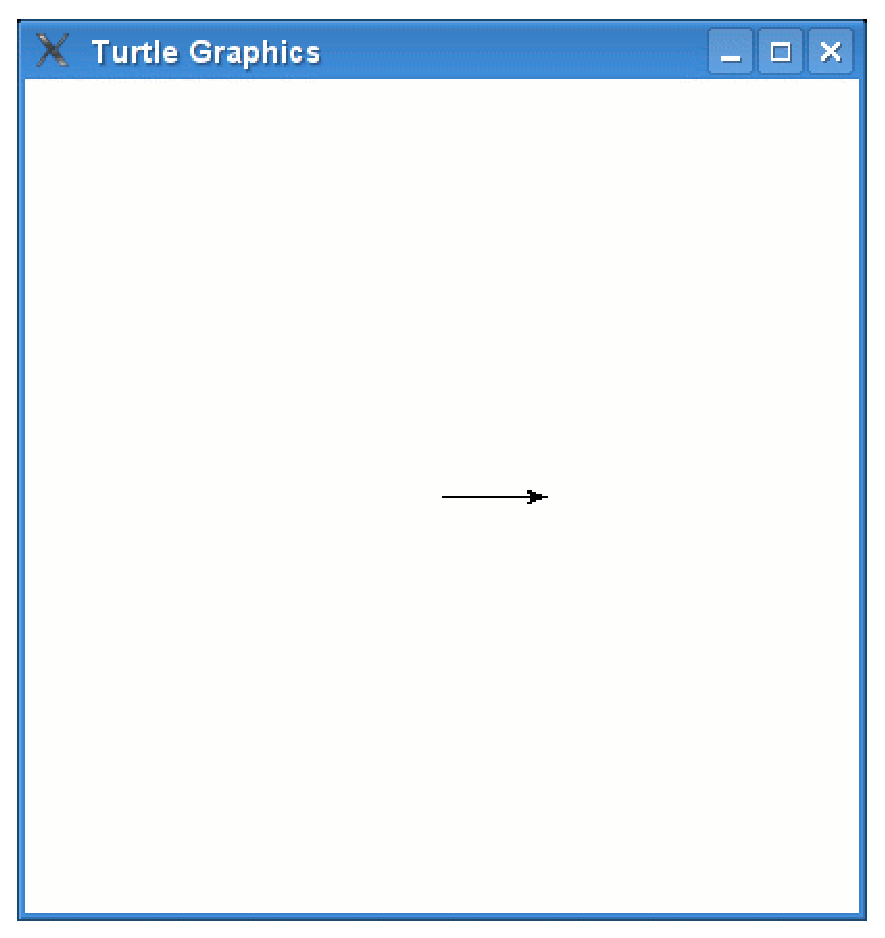
\includegraphics[width=72mm]{eps/figure11.eps}
\end{center}
\caption{The turtle draws a line.}\label{fig11}
\end{figure}

From the turtle's point-of-view, she has moved forward 50 steps.  From our point-of-view, she has moved 50 pixels.

\noindent
\emph{So, what's a pixel?}

A pixel\index{pixels} is a dot on the screen.  When you look at your computer, everything is made up of tiny (square) dots.  The programs you use and the games you play on the computer, or with a Playstation, or an Xbox, or a Wii; are all made up of a whole bunch of different coloured dots, arranged on the screen.  In fact, if you look at your computer screen with a magnifying glass, you might just be able to make out some of those dots. So if we zoom in on the canvas and the line that was just drawn by the turtle, we can see the arrow representing the turtle, is also just a bunch of square dots, as you can see in figure~\ref{fig12}.

\begin{figure}
\begin{center}
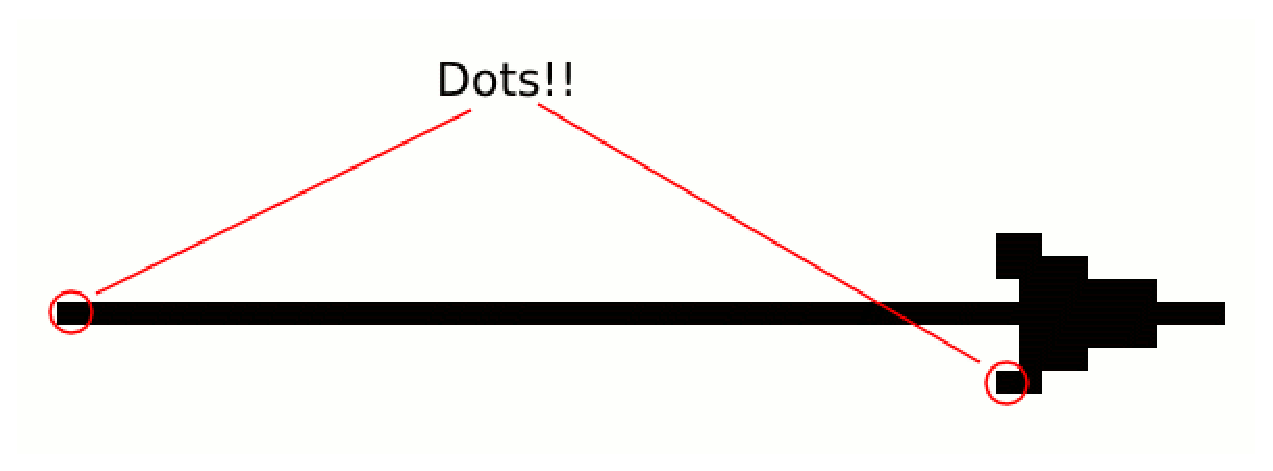
\includegraphics[width=72mm]{eps/figure12.eps}
\end{center}
\caption{Zooming in on the line and the arrow.}\label{fig12}
\end{figure}

We'll talk more about these dots, or pixels, in a later chapter.

Next, we can tell the turtle to turn left\index{turtle!turning left} or right\index{turtle!turning right}:

\begin{listing}
\begin{verbatim}
>>> t.left(90)
\end{verbatim}
\end{listing}

This tells the turtle to turn left, 90 degrees.  You may not have learned about degrees\index{degrees} in school so far, but the easiest way to think about them, is that they are like the divisions on the face of a clock as seen in figure~\ref{fig13}.

\begin{figure}
\begin{center}
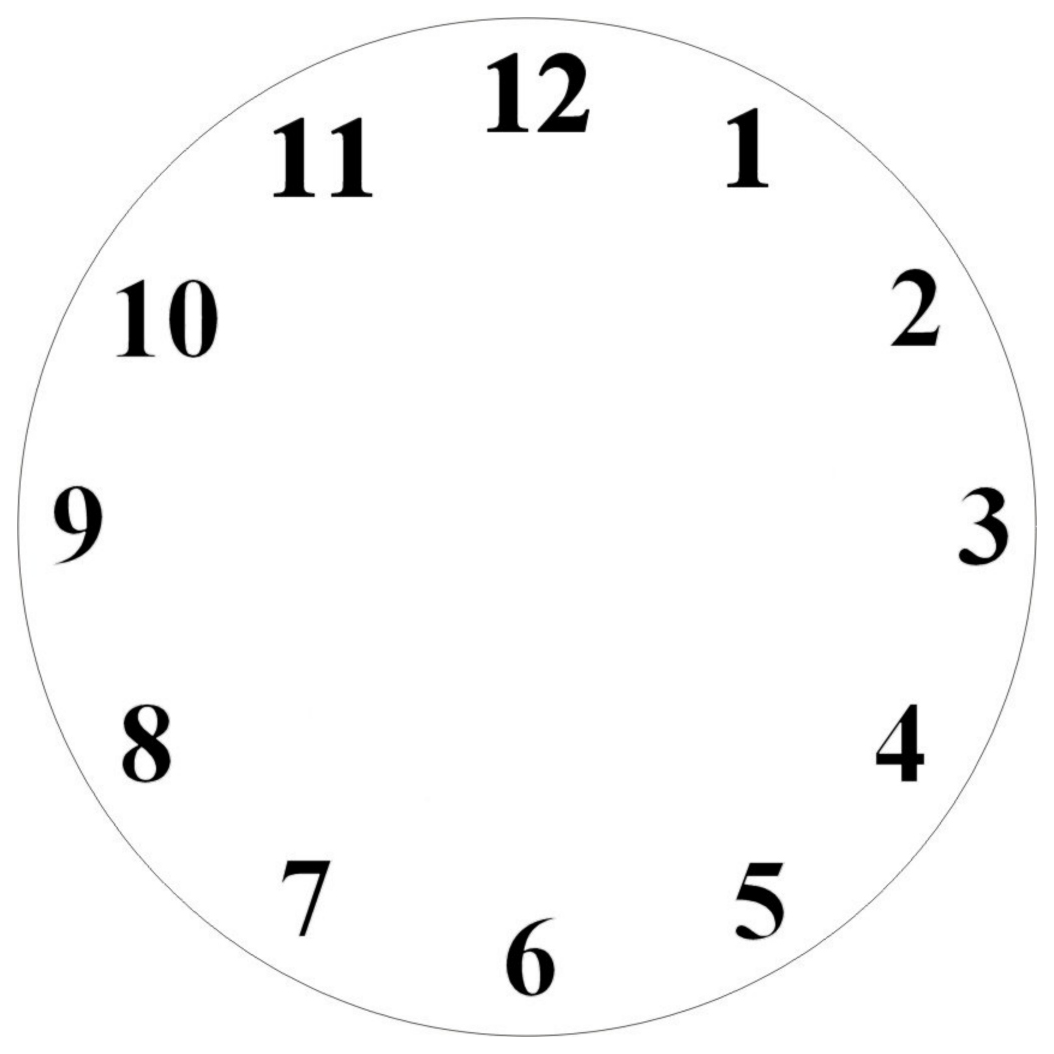
\includegraphics[width=52mm]{eps/figure13.eps}
\end{center}
\caption{The `divisions' on a clock.}\label{fig13}
\end{figure}

The difference to a clock, is that rather than 12 divisions (or 60, if you're counting minutes rather than hours), there are 360 divisions.  So, if you count 360 divisions around the face of a clock, you get 90 where there's normally a 3, 180 where there's normally a 6, and 270 where there's normally a 9; and 0 would be at the top (at the start), where you normally see a 12.  Figure~\ref{fig14} shows you the degree divisions.

\begin{figure}
\begin{center}
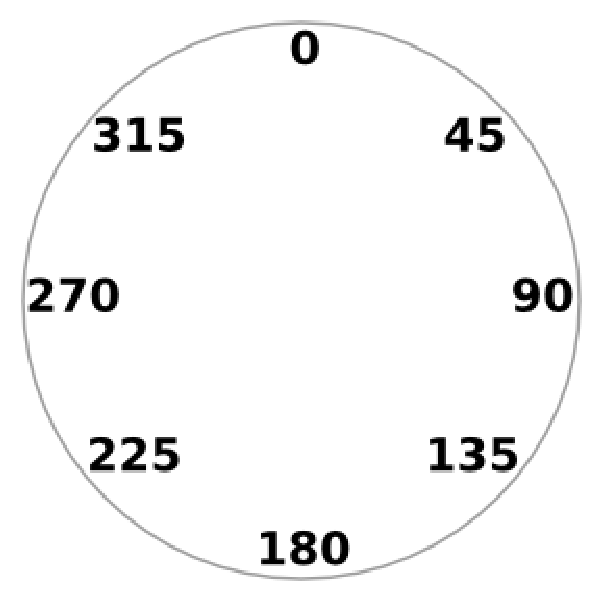
\includegraphics[width=52mm]{eps/figure14.eps}
\end{center}
\caption{Degrees.}\label{fig14}
\end{figure}

So, what does it actually mean when you call \code{left(90)}?
\par
If you stand and face one direction, point your arm out directly away from your shoulder, THAT is 90 degrees.  If you point your left arm, that's 90 degrees left.  If you point your right arm, that's 90 degrees right.  When Python's turtle turns left, she plants her nose in one spot then swivels her body around the face the new direction (same as if you turned your body to face where your arm is pointing).  So, \code{t.left(90)} results in the arrow now pointing upwards, as shown in figure~\ref{fig15}.

\begin{figure}
\begin{center}
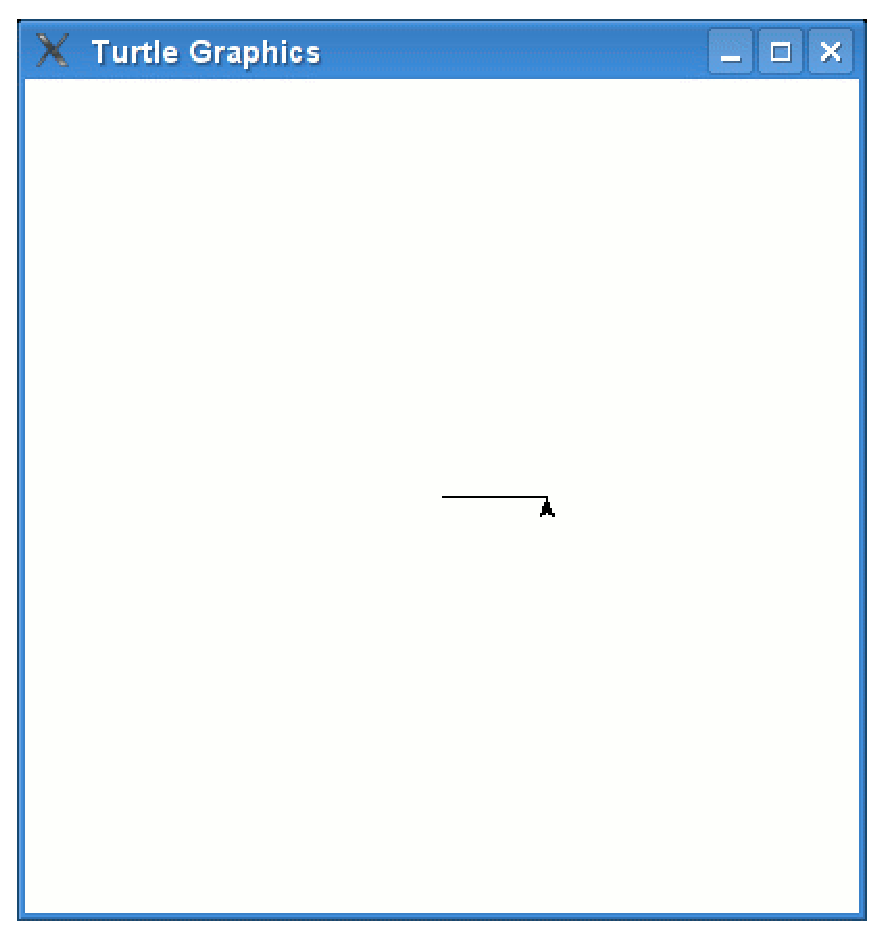
\includegraphics[width=72mm]{eps/figure15.eps}
\end{center}
\caption{The turtle after turning left.}\label{fig15}
\end{figure}

Let's try the same commands again a few times:

\begin{listing}
\begin{verbatim}
>>> t.forward(50)
>>> t.left(90)
>>> t.forward(50)
>>> t.left(90)
>>> t.forward(50)
>>> t.left(90)
\end{verbatim}
\end{listing}

Our turtle has drawn a square and is left facing the same direction as she started (see figure~\ref{fig16}).

\begin{figure}
\begin{center}
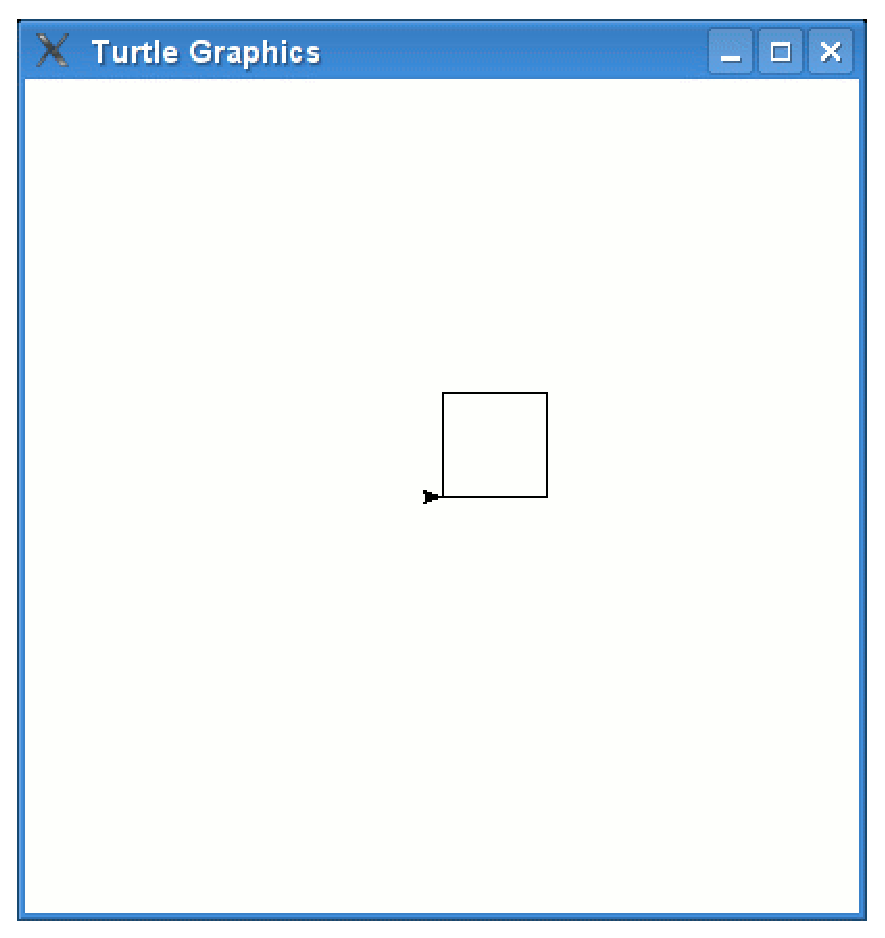
\includegraphics[width=72mm]{eps/figure16.eps}
\end{center}
\caption{Drawing a square.}\label{fig16}
\end{figure}

We can erase what's on the canvas by using clear\index{turtle!clear}:

\begin{listing}
\begin{verbatim}
>>> t.clear()
\end{verbatim}
\end{listing}

Some of the other basic functions you can use with your turtle are: \code{reset}\index{turtle!reset}, which also clears the screen, but puts the turtle automatically back into her starting position; \code{backward}\index{turtle!backward}, which moves the turtle backwards; \code{right}, which turns the turtle to the right; \code{up}\index{turtle!up (stop drawing)} which tells the turtle to stop drawing as she moves (in other words pick her pen up off the canvas); and finally \code{down}\index{turtle!down (start drawing)} which tells the turtle to start drawing again. You call these functions in the same way we've used the others:

\begin{listing}
\begin{verbatim}
>>> t.reset()
>>> t.backward(100)
>>> t.right(90)
>>> t.up()
>>> t.down()
\end{verbatim}
\end{listing}

\noindent
We'll come back to the turtle module shortly.

\section{Things to try}

\emph{In this chapter we saw how to use turtle to draw simple lines, using left and right turns.  We saw that turtle uses degrees to turn, a bit like the minute divisions on a clock face.}

\subsection*{Exercise 1}
Create a canvas using turtle's \code{Pen} function, and draw a rectangle.

\subsection*{Exercise 2}
Create another canvas using turtles \code{Pen} function, and draw a triangle.

\newpage
